\documentclass[a4paper]{article}
\usepackage{graphicx}
\usepackage{subcaption}
\usepackage[a4paper]{geometry}
\geometry{margin=1.5cm}
\usepackage{multicol}
% TODO: color url 
\usepackage{hyperref}
\hypersetup{colorlinks=false,urlcolor=blue}
\usepackage{array}
\usepackage{enumitem}

%TODO typing Greek in Latex???

\begin{document}
\title{Authorship Attribution based on Stylistic Analysis of Particle Distribution}
\author{Andreas Linz, Ute Tischer, Stylianos Chronopoulos, Ying-Chi Lin, Huan Meng}
\date{March 2015}
\maketitle

\section{Introduction}
Since the motivation of this project is already presented in the presentation, we do not wish to be repetitious here. In this report, we mainly focus on details of our solution process and presenting the analysis results. \\

In the analyses, the first two numbers of each file name used in sblgnt data source are taken to represent each letter. Pauline letters are grouped into three categories: \\
\begin{itemize}
\item Letters confirmed to be written by Paul: 66, 67, 68, 69, 71, 73, 78 
\item Letters confirmed to be NOT written by Paul: 75, 76, 77, 79 
\item Letters not certain if is written by Paul: 70, 72, 74
\end{itemize}

The Petrine letters are noted as 81 and 82. \\

\section{Data Extraction - sblgntparser}
To make it easy to do queries on our data set, the \href{https://github.com/morphgnt/sblgnt}{SBL Greek New Testament}, we needed to parse it and enrich the outcoming data structure with more information, like the position of a word in a sentence. \\
Luckily, the SBLGNT format stores a lot of information for every word in each of the books. Each book of the Greek New Testament is saved as one or more text files, where each file consists of a number of rows and each row describes a word in the book. An example row looks like this: \\

%TODO GREEK LETTERS!!
010101 N- ----NSF-\textgreek{?????? ?????? ?????? ??????}

The first six digits are three pairs of two numbers each, they store the book, chapter and verse where the word in this row occurs in the book. The next two characters encode the part of speech of the word, in this example the word is a noun. Thereafter are the codes that describe certain features of a word, like person, tense, mood, degree and so on. We had to reverse engineer the meaning of the codes, with the help of  \href{http://jtauber.com/2010/07/parse-helper/demo.html}{this tool}, because there was no description available or we haven�t found it. The last four words in the row are different forms of the word, the text, word, normalized and lemma form. We only used the lemma form for our queries because this is the one that is the same for different shapes of the same word. \\

While parsing the data set, I enriched each word in the data model with their position in the sentence (remember there is only the verse encoded in the source), the position in the whole text, the distance to the next in-sentence punctuation (g.e. commata) and each word was linked to its neighbours in the sentence. This gave us the possibility to reason about words based on the type and form of their surrounding words.  \\

The \href{https://github.com/KLINGTdotNET/sblgntparser/blob/master/sblgntparser/model.py}{data model}, in which the parsed text is transformed into, consists of mainly three parts, these are the text, sentence and word object. Each object has different methods that you can use to ask questions on the text, g.e. loop over all words in the text and return only the conjunctions. Our goal was to do an authorship attribution based on particle distribution, so we needed to make queries on the particles in the text. Because the particle type was not encoded directly in the SBLGNT we had to use list of all ancient greek particles to find them in the text. 

\newpage
\section{Data Analysis - absolute position analysis}
With the help of sblgntparser, the following variables of data are extracted from the sblgnt text for later analyses:
\begin{enumerate}[itemsep=-1mm]
\item sample\_no: one number for each data row
\item letter: first two digits of the source file name, for identification
\item author: name of (likely) author
\item authenticity: categories in wikipedia, coding is \href{https://github.com/KLINGTdotNET/dh-project-ws14/blob/master/data/paul_letters.txt}{here}.
\item particle
\item part of speech (POS) of the particle
\item position from the start of the sentence
\item position from the end of the sentence
\item left neighbor of the particle
\item POS of left neighbor
\item right neighbor of the particle
\item POS of right neighbor
\item previous in-sentence (PIP) punctuation and the word 
\item PIP position (from sentence start)
\item following in-sentence punctuation (FIP) and the word
\item FIP position (from sentence start)
\end{enumerate}

% SEMICOLON NOT SHOWN
\noindent For the parsing, sentences are defined as text (including in-sentence punctuations) separated by period ( . ), comma ( , ) and greek question mark ( ; ). In-sentence punctuations are semicolon ( � ) and comma ( , ). 

All the particle occurrences in every corpus and their relevant fields mentioned above are extracted using Python. The results are available at: \href{https://github.com/KLINGTdotNET/dh-project-ws14/tree/master/data/output/paul_par}{Paul�s letters} and \href{https://github.com/KLINGTdotNET/dh-project-ws14/tree/master/data/output/peter_par}{Peter�s letters}.

\subsection{Absolute position analysis}
Generally speaking, when a particle is rarely used and has very strict syntax rule so that position variation in a sentence is hardly possible, it is less suitable for stylometric analysis. In the search of suitable particles in the corpus, in addition to extract the overall frequency of each particle in all sample letters, visualisation of the absolute positions of each particle in each letter is also carried out.  

\subsection{Visualisation of absolute position analysis}
Absolute position of a particle is defined as the position of the particle from the nearest previous punctuation which includes sentence separating punctuation and in-sentence punctuation (PIP). For each particle, its frequency (\textit{number of occurrence in the letter}) in each absolute position is extracted using Python. Furthermore, its position distribution is calculated as (\textit{number of occurrence in each position})/(\textit{total occurrence of the particle in the letter}). The frequency-position plots for each particle in each letter are drawn using R. To distinguish between types of absolute positions, yellow color is used to depict absolute positions from the start of a sentence and green is for absolute position after a PIP. The quellcodes for frequency extraction are on \href{https://github.com/KLINGTdotNET/dh-project-ws14/tree/master/src/absolute_freq}{this page}. \\

\noindent In file �run.sh� contains the workflow of the frequency extraction and plotting, with some batch files in between to connect the subprocesses. For easier comparison, plots are grouped by particles and output as PDF files. 

\subsection{Selection of particles}
Particles with a minimum occurrence in the corpus and with suitable variations in terms of their absolute positions are those we aim for. The following describes the selection by these two criteria:

\paragraph{by frequency} 
for each author, the frequencies of every particle in each letter and their overall occurrence in all letters are shown in Table 1. Particles occur most frequently in Paul�s letters correspondent to those in Peter�s letters and the rankings of occurrence are also identical between both authors. Based on the this frequency results,  particles ???(kai), ???(de) and ???(yap) are selected for absolute position analysis. \\

%TODO Greek letters
{\renewcommand{\arraystretch}{1.3}
\begin{tabular}{ccc}
\hline
Particle &	\multicolumn{2}{c}{Frequency} \\
\cline{2-3}
&in Pauline letters  & in Petrine letters \\
\hline
??? & 1406 & 108 \\
??	& 696 & 49 \\
???	& 546 &25 \\
????	 & 327&22 \\
???	& 123 &7 \\
???  & 71 & 4 \\
??    & 44&	\\
???  & 29	& \\
??    & 22	& \\
????????? & 2	& \\
?????? &	2& \\	
???  & 1	& \\
?????? & 1 &\\
?????? & 1&	\\
\hline
\end{tabular}
}

% TODO Greek letters
\paragraph{by absolute position variation}
???(kai) (engl. and) is the most frequent particle of all. Its absolute position in each letter can be seen in Figure \ref{paul_kai} and \ref{peter_kai}. In most letters of Paul, ???(kai) occurs most frequently at position one, with frequency distribution ranges from 15.6\%  to 42.7\%. Three exceptions with most dominant position at position five are letters 75, 77 and 78. Letters 77 and 78 have the least ???(kai) occurrence (34 and 13 counts, respectively) and letter 78 has moderate frequent of ???(kai) (83 counts). The two letters from Peter show also the same patterns, in letter 79, 39\% of the occurrence are at position one and with a small total count of 13, ???(kai) occurs most frequency in position two in letter 78. Since letter 78 is confirmed to be written by Paul and letters 75 and 77 are categorized as uncertain by Paul and additionally, both patterns are observed by two Peter�s letters, leads to the conclusion that the observed patterns of ???(kai) is not distinct for identification of authorship.
???(de), the second most frequent particles of all, always dominant at position 2 in all letters (Figure \ref{paul_de} and \ref{peter_de}). Same pattern is observed with ???(kai) with mostly at least 80\% of the occurrence at position two. Little variations on dominant position of ???(yap) is also seen (Figure \ref{paul_yap} and \ref{peter_yap}). Therefore, these three particles do not indicate obvious difference between two authors or between different categories of Paul�s letters. 

The analysis results show that little absolute position variation is observed in the most of the most frequent particles, ???(kai), ???(de) and ???(yap),  in the corpus. Though ???(kai) occurs in more positions in the sentences, its variation in position distribution can be due to small sample size than authorship difference. Therefore, in order to get more accurate results, longer text and larger corpus is recommended to be used. 

\begin{figure}
\begin{subfigure}{0.45\textwidth}
\centering
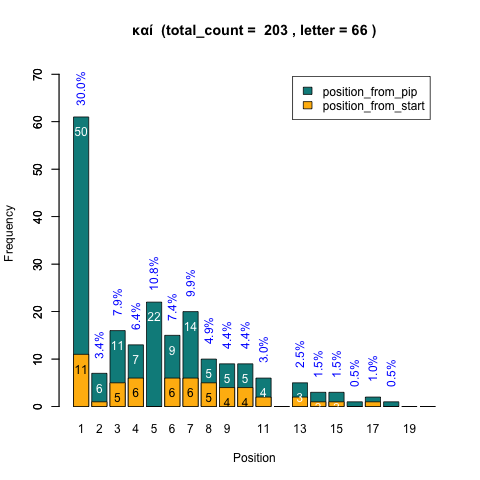
\includegraphics[width=1\linewidth]{paul_plots/par3_lt66.png}
\end{subfigure}
\begin{subfigure}{0.45\textwidth}
\centering
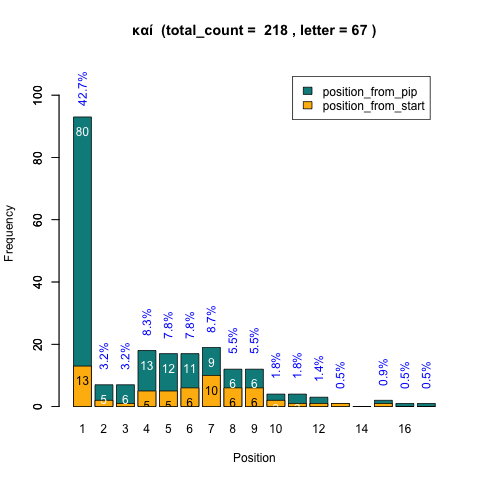
\includegraphics[width=1\linewidth]{paul_plots/par3_lt67.png}
\end{subfigure}
\begin{subfigure}{0.45\textwidth}
\centering
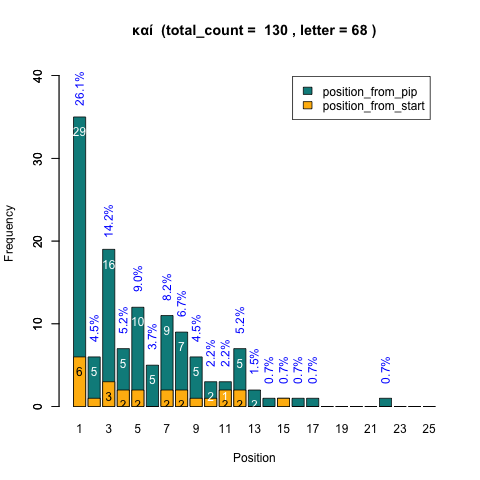
\includegraphics[width=1\linewidth]{paul_plots/par3_lt68.png}
\end{subfigure}
\begin{subfigure}{0.45\textwidth}
\centering
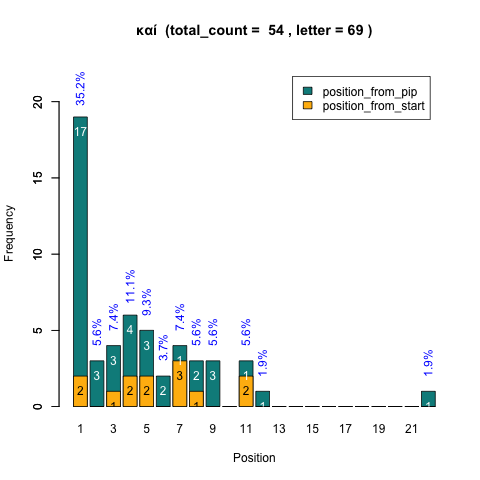
\includegraphics[width=1\linewidth]{paul_plots/par3_lt69.png}
\end{subfigure}
\begin{subfigure}{0.45\textwidth}
\centering
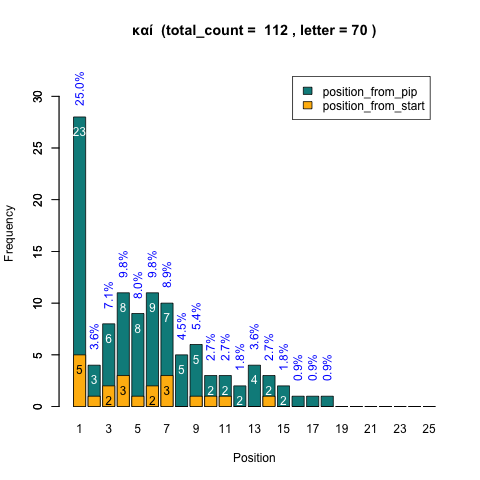
\includegraphics[width=1\linewidth]{paul_plots/par3_lt70.png}
\end{subfigure}
\begin{subfigure}{0.45\textwidth}
\centering
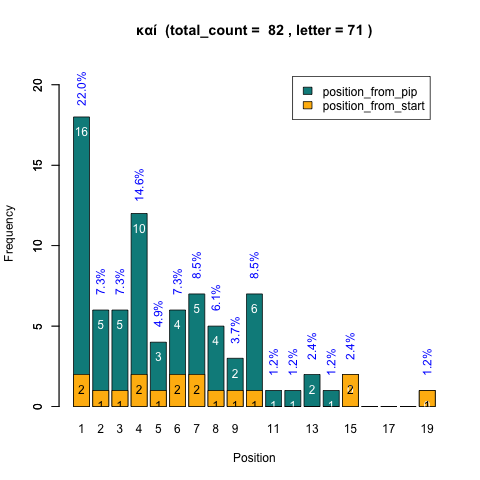
\includegraphics[width=1\linewidth]{paul_plots/par3_lt71.png}
\end{subfigure}
\caption{Frequency of particle ???(kai) at each absolute position in Pauline letters}
\label{paul_kai}
\end{figure}

\begin{figure}
\ContinuedFloat
\begin{subfigure}{0.45\textwidth}
\centering
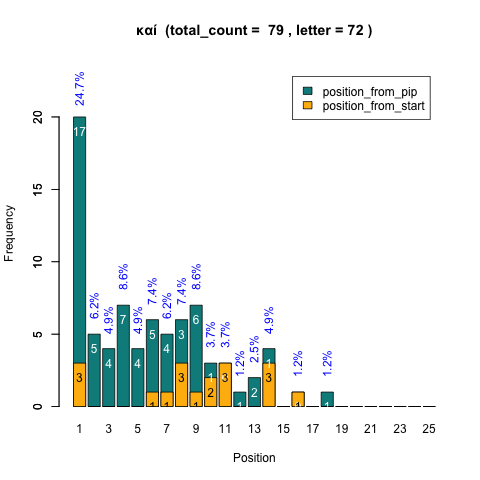
\includegraphics[width=1\linewidth]{paul_plots/par3_lt72.png}
\end{subfigure}
\begin{subfigure}{0.45\textwidth}
\centering
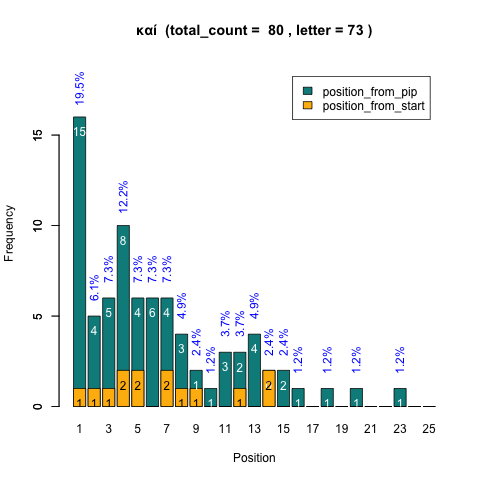
\includegraphics[width=1\linewidth]{paul_plots/par3_lt73.png}
\end{subfigure}
\begin{subfigure}{0.45\textwidth}
\centering
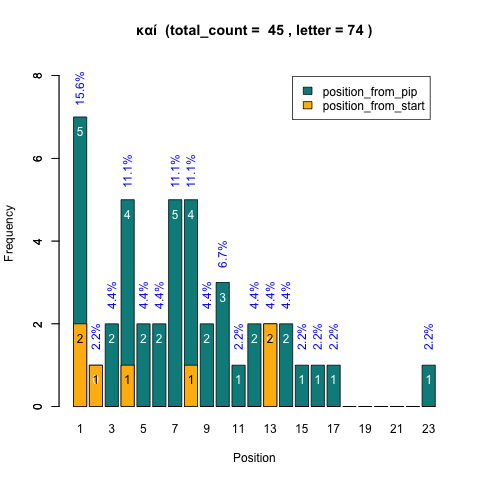
\includegraphics[width=1\linewidth]{paul_plots/par3_lt74.png}
\end{subfigure}
\begin{subfigure}{0.45\textwidth}
\centering
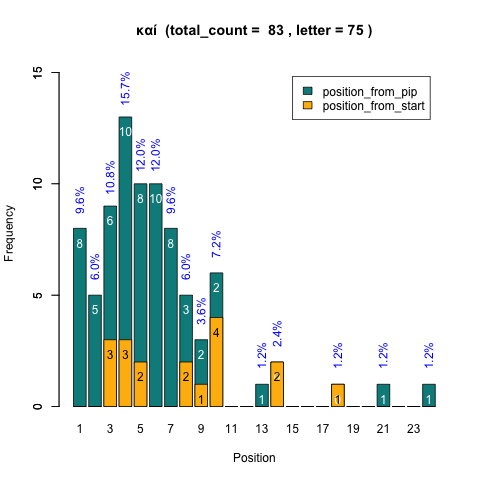
\includegraphics[width=1\linewidth]{paul_plots/par3_lt75.png}
\end{subfigure}
\begin{subfigure}{0.45\textwidth}
\centering
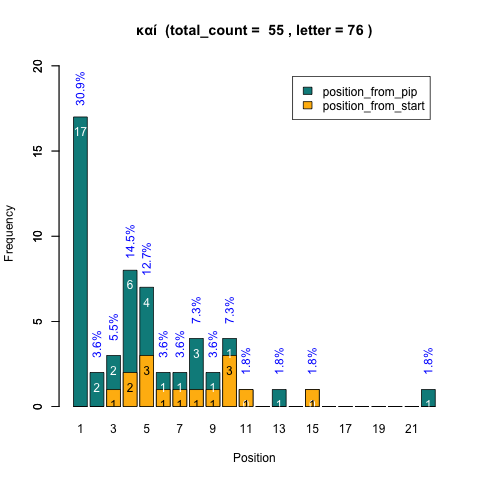
\includegraphics[width=1\linewidth]{paul_plots/par3_lt76.png}
\end{subfigure}
\begin{subfigure}{0.45\textwidth}
\centering
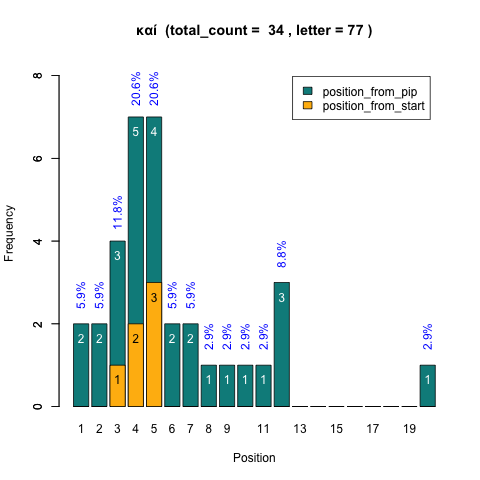
\includegraphics[width=1\linewidth]{paul_plots/par3_lt77.png}
\end{subfigure}
\caption{Frequency of particle ???(kai) at each absolute position in Pauline letters}
\end{figure}

\begin{figure}
\ContinuedFloat
\begin{subfigure}{0.45\textwidth}
\centering
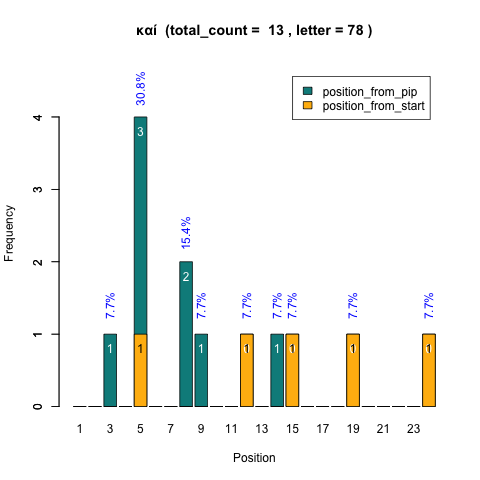
\includegraphics[width=1\linewidth]{paul_plots/par3_lt78.png}
\end{subfigure}
\begin{subfigure}{0.45\textwidth}
\centering
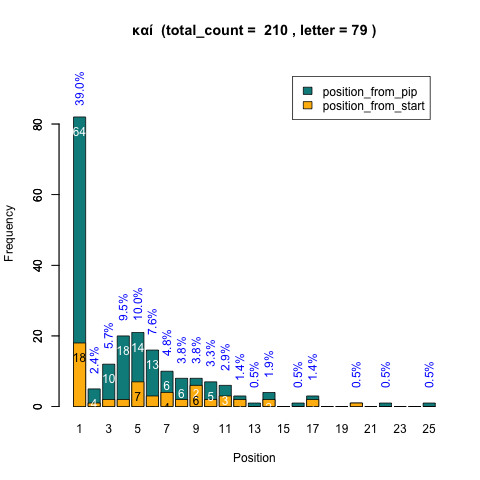
\includegraphics[width=1\linewidth]{paul_plots/par3_lt79.png}
\end{subfigure}
\caption{Frequency of particle ???(kai) at each absolute position in Pauline letters}
\end{figure}

\begin{figure}
\begin{subfigure}{0.45\textwidth}
\centering
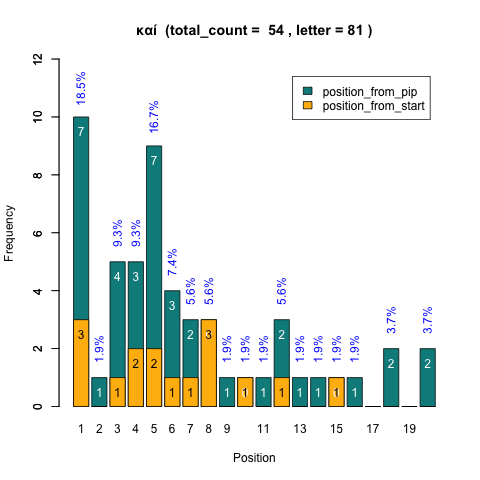
\includegraphics[width=1\linewidth]{peter_plots/par3_lt81.png}
\end{subfigure}
\begin{subfigure}{0.45\textwidth}
\centering
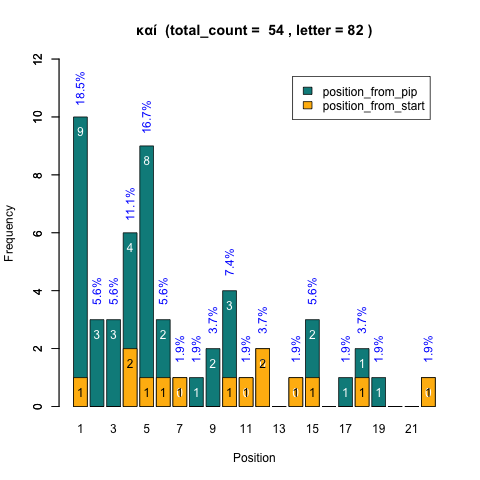
\includegraphics[width=1\linewidth]{peter_plots/par3_lt82.png}
\end{subfigure}
\caption{Frequency of particle ???(kai) at each absolute position in petrine letters}
\label{peter_kai}
\end{figure}

\begin{figure}
\begin{subfigure}{0.45\textwidth}
\centering
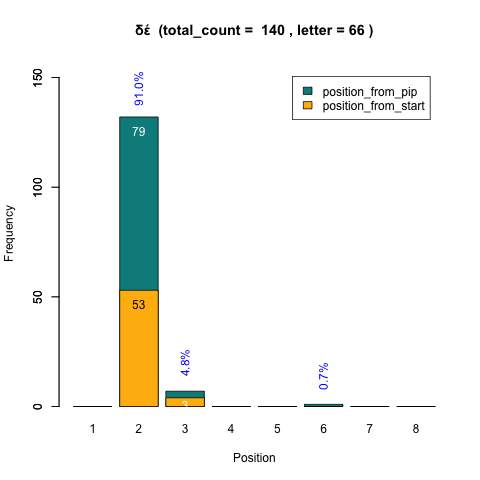
\includegraphics[width=1\linewidth]{paul_plots/par2_lt66.png}
\end{subfigure}
\begin{subfigure}{0.45\textwidth}
\centering
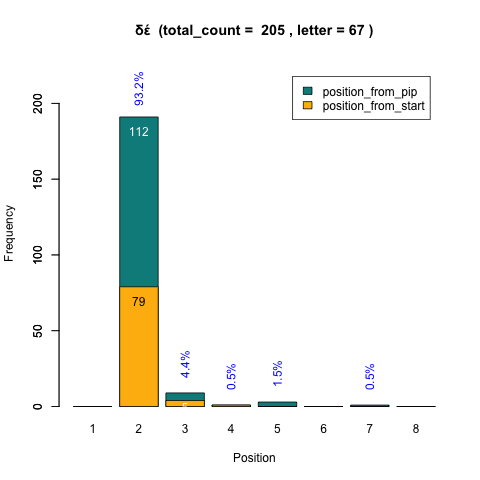
\includegraphics[width=1\linewidth]{paul_plots/par2_lt67.png}
\end{subfigure}
\begin{subfigure}{0.45\textwidth}
\centering
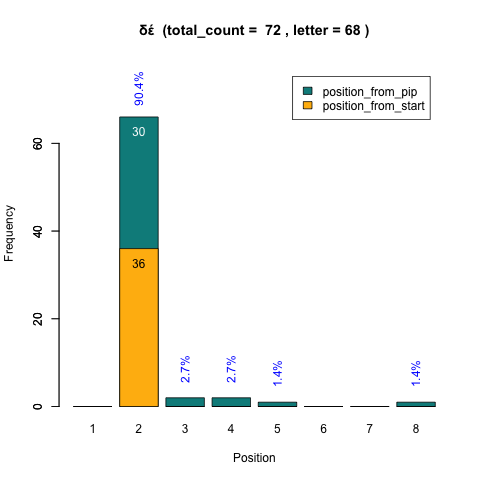
\includegraphics[width=1\linewidth]{paul_plots/par2_lt68.png}
\end{subfigure}
\begin{subfigure}{0.45\textwidth}
\centering
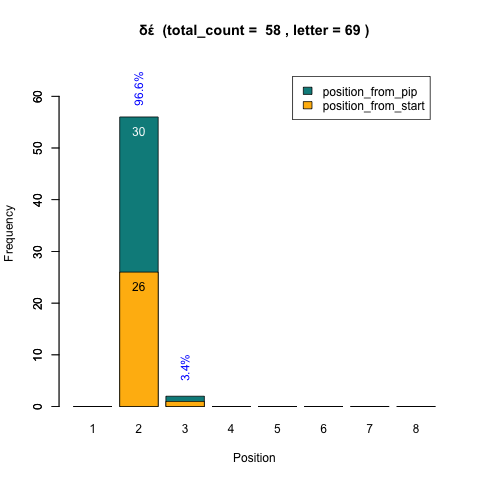
\includegraphics[width=1\linewidth]{paul_plots/par2_lt69.png}
\end{subfigure}
\begin{subfigure}{0.45\textwidth}
\centering
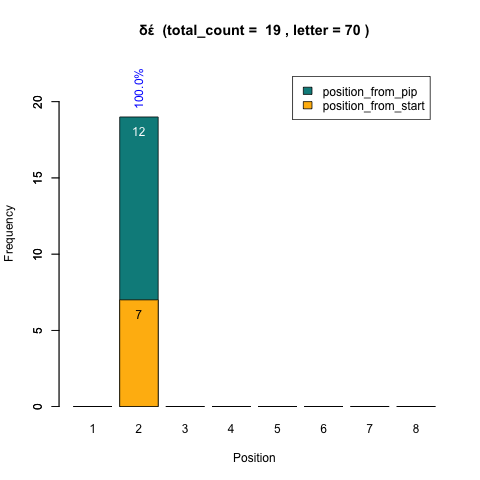
\includegraphics[width=1\linewidth]{paul_plots/par2_lt70.png}
\end{subfigure}
\begin{subfigure}{0.45\textwidth}
\centering
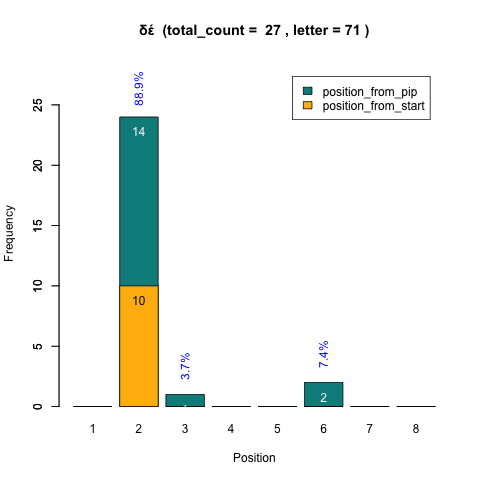
\includegraphics[width=1\linewidth]{paul_plots/par2_lt71.png}
\end{subfigure}
\caption{Frequency of particle ???(de) at each absolute position in Pauline letters}
\label{paul_de}
\end{figure}

\begin{figure}
\ContinuedFloat
\begin{subfigure}{0.45\textwidth}
\centering
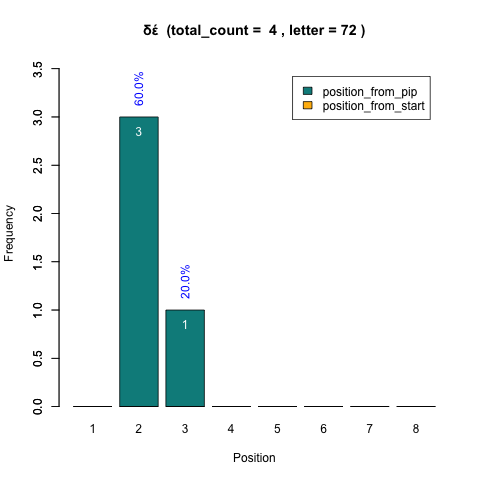
\includegraphics[width=1\linewidth]{paul_plots/par2_lt72.png}
\end{subfigure}
\begin{subfigure}{0.45\textwidth}
\centering
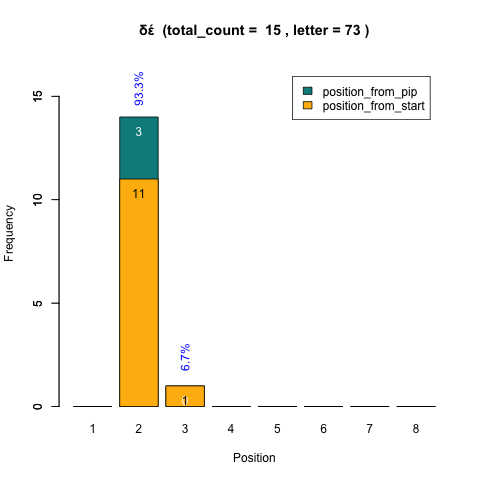
\includegraphics[width=1\linewidth]{paul_plots/par2_lt73.png}
\end{subfigure}
\begin{subfigure}{0.45\textwidth}
\centering
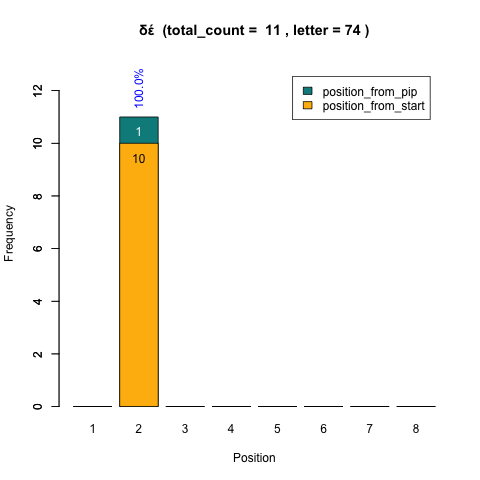
\includegraphics[width=1\linewidth]{paul_plots/par2_lt74.png}
\end{subfigure}
\begin{subfigure}{0.45\textwidth}
\centering
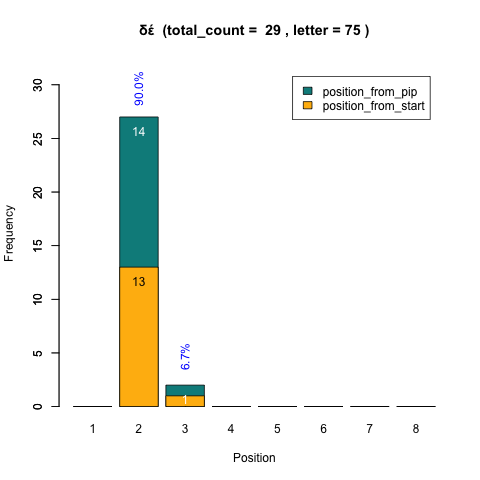
\includegraphics[width=1\linewidth]{paul_plots/par2_lt75.png}
\end{subfigure}
\begin{subfigure}{0.45\textwidth}
\centering
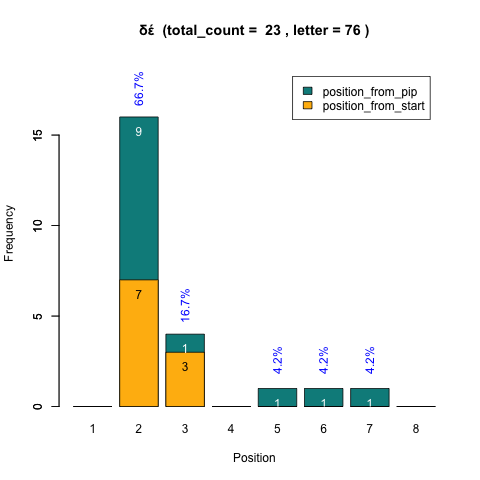
\includegraphics[width=1\linewidth]{paul_plots/par2_lt76.png}
\end{subfigure}
\begin{subfigure}{0.45\textwidth}
\centering
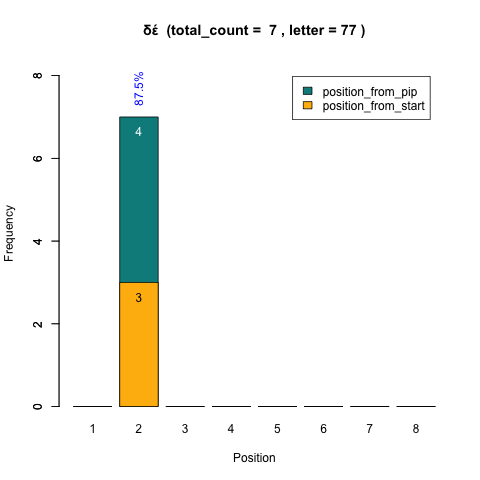
\includegraphics[width=1\linewidth]{paul_plots/par2_lt77.png}
\end{subfigure}
\caption{Frequency of particle ???(de) at each absolute position in Pauline letters}
\end{figure}

\begin{figure}
\ContinuedFloat
\begin{subfigure}{0.45\textwidth}
\centering
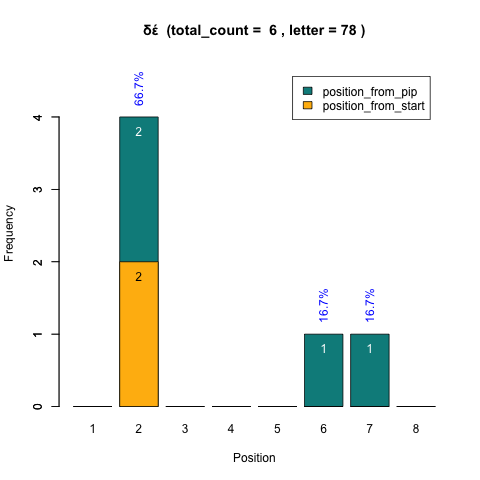
\includegraphics[width=1\linewidth]{paul_plots/par2_lt78.png}
\end{subfigure}
\begin{subfigure}{0.45\textwidth}
\centering
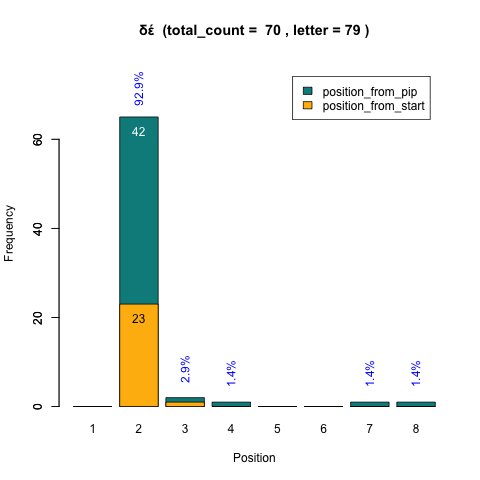
\includegraphics[width=1\linewidth]{paul_plots/par2_lt79.png}
\end{subfigure}
\caption{Frequency of particle ???(de) at each absolute position in Pauline letters}
\end{figure}

\begin{figure}
\begin{subfigure}{0.45\textwidth}
\centering
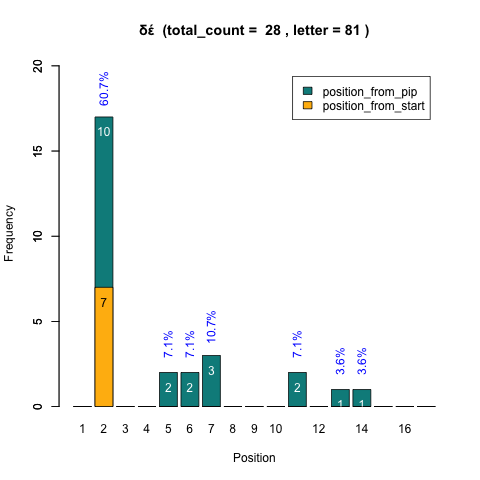
\includegraphics[width=1\linewidth]{peter_plots/par2_lt81.png}
\end{subfigure}
\begin{subfigure}{0.45\textwidth}
\centering
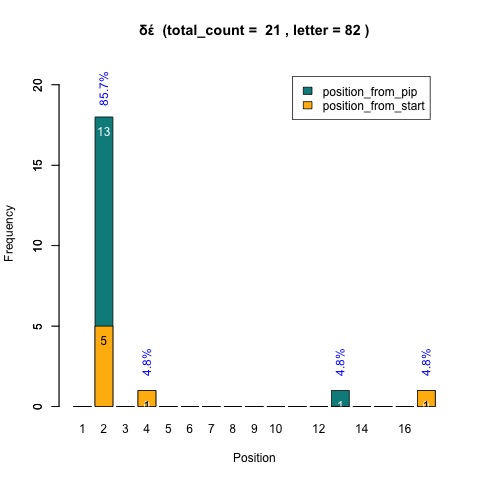
\includegraphics[width=1\linewidth]{peter_plots/par2_lt82.png}
\end{subfigure}
\caption{Frequency of particle ???(de) at each absolute position in petrine letters}
\label{peter_de}
\end{figure}

\begin{figure}
\begin{subfigure}{0.45\textwidth}
\centering
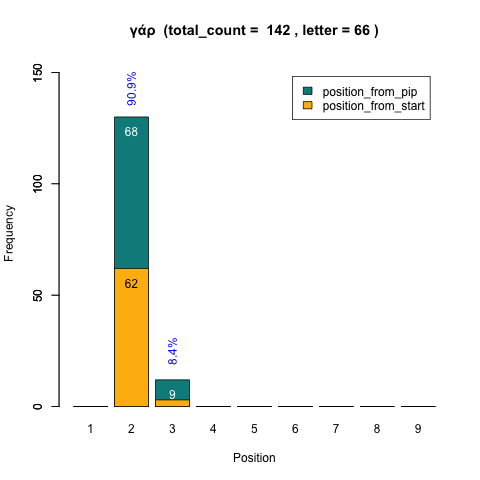
\includegraphics[width=1\linewidth]{paul_plots/par1_lt66.png}
\end{subfigure}
\begin{subfigure}{0.45\textwidth}
\centering
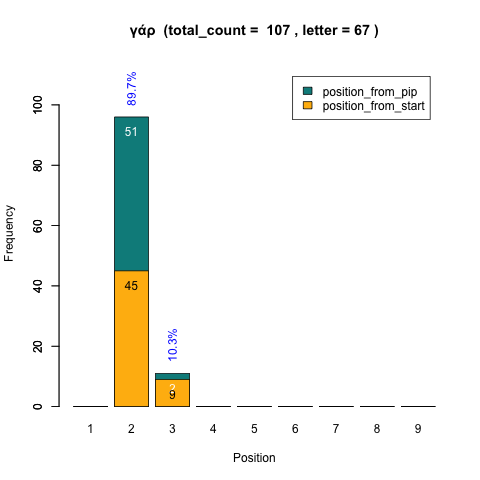
\includegraphics[width=1\linewidth]{paul_plots/par1_lt67.png}
\end{subfigure}
\begin{subfigure}{0.45\textwidth}
\centering
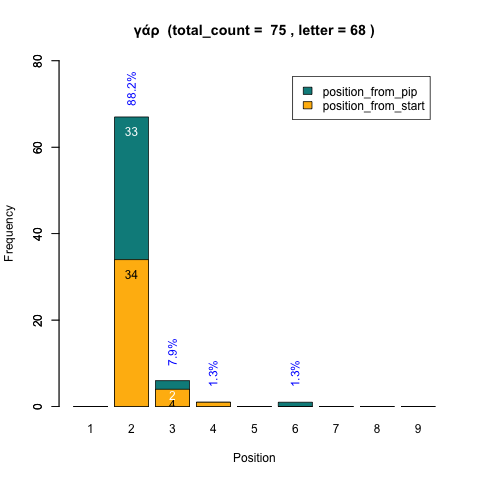
\includegraphics[width=1\linewidth]{paul_plots/par1_lt68.png}
\end{subfigure}
\begin{subfigure}{0.45\textwidth}
\centering
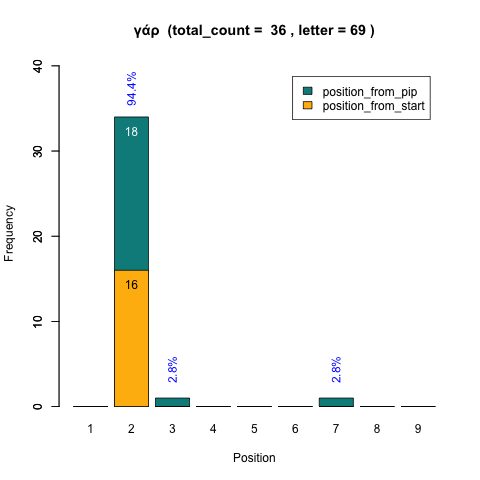
\includegraphics[width=1\linewidth]{paul_plots/par1_lt69.png}
\end{subfigure}
\begin{subfigure}{0.45\textwidth}
\centering
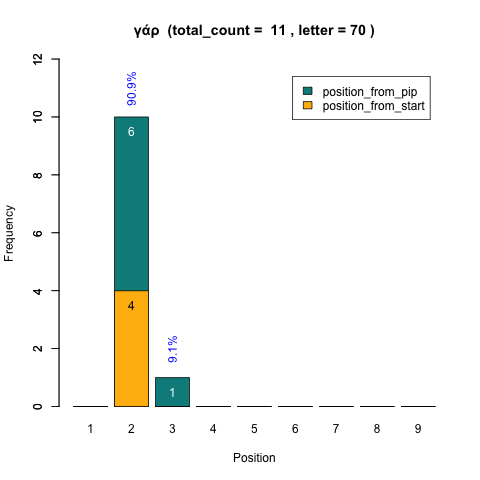
\includegraphics[width=1\linewidth]{paul_plots/par1_lt70.png}
\end{subfigure}
\begin{subfigure}{0.45\textwidth}
\centering
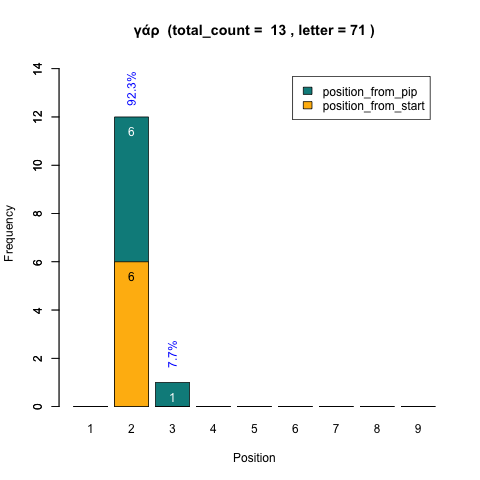
\includegraphics[width=1\linewidth]{paul_plots/par1_lt71.png}
\end{subfigure}
\caption{Frequency of particle ???(yap) at each absolute position in Pauline letters}
\label{paul_yap}
\end{figure}

\begin{figure}
\ContinuedFloat
\begin{subfigure}{0.45\textwidth}
\centering
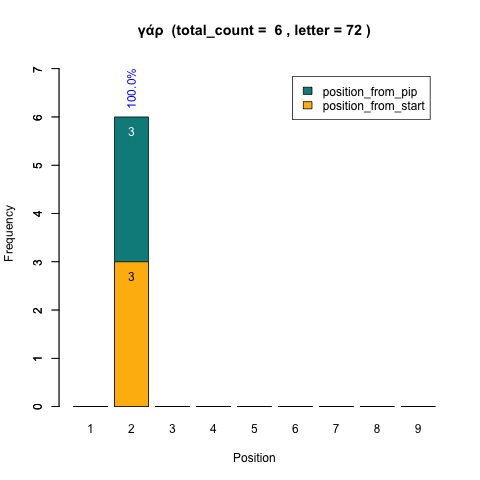
\includegraphics[width=1\linewidth]{paul_plots/par1_lt72.png}
\end{subfigure}
\begin{subfigure}{0.45\textwidth}
\centering
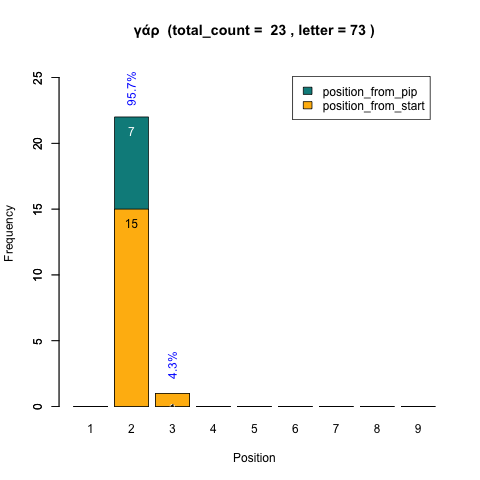
\includegraphics[width=1\linewidth]{paul_plots/par1_lt73.png}
\end{subfigure}
\begin{subfigure}{0.45\textwidth}
\centering
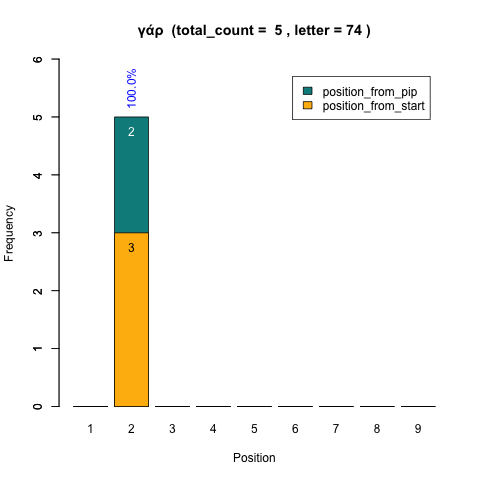
\includegraphics[width=1\linewidth]{paul_plots/par1_lt74.png}
\end{subfigure}
\begin{subfigure}{0.45\textwidth}
\centering
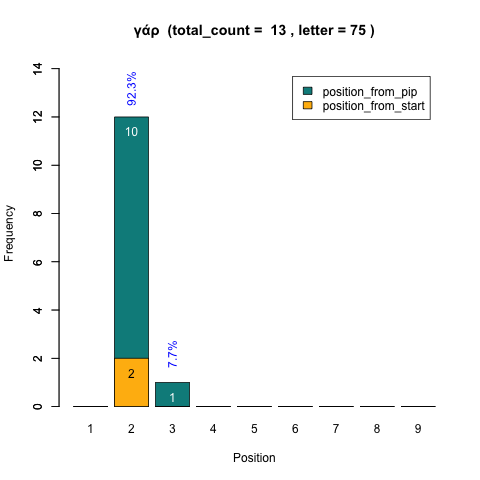
\includegraphics[width=1\linewidth]{paul_plots/par1_lt75.png}
\end{subfigure}
\begin{subfigure}{0.45\textwidth}
\centering
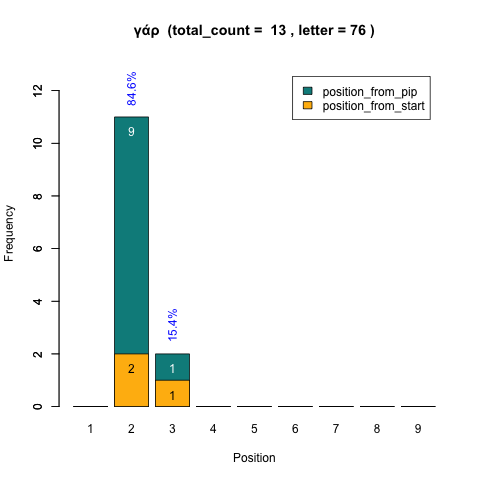
\includegraphics[width=1\linewidth]{paul_plots/par1_lt76.png}
\end{subfigure}
\begin{subfigure}{0.45\textwidth}
\centering
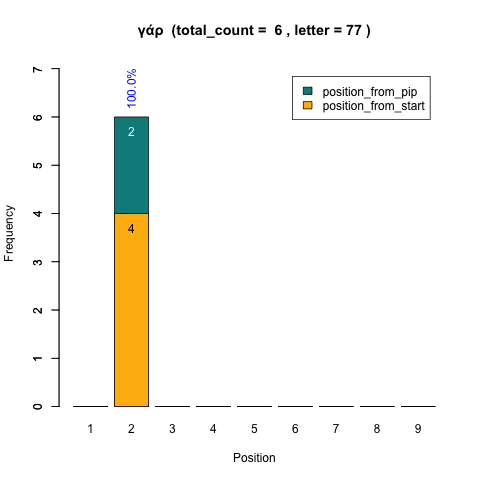
\includegraphics[width=1\linewidth]{paul_plots/par1_lt77.png}
\end{subfigure}
\caption{Frequency of particle ???(yap) at each absolute position in Pauline letters}
\end{figure}

\begin{figure}
\ContinuedFloat
\begin{subfigure}{0.45\textwidth}
\centering
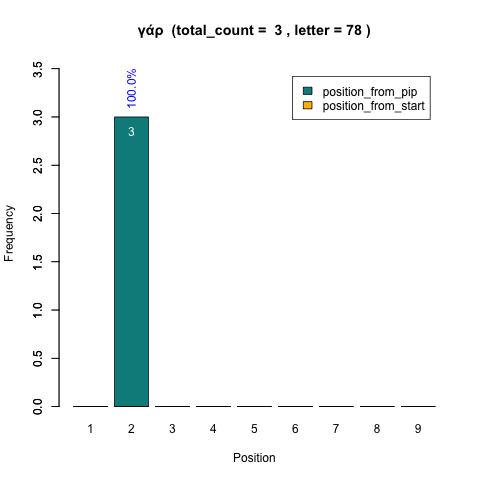
\includegraphics[width=1\linewidth]{paul_plots/par1_lt78.png}
\end{subfigure}
\begin{subfigure}{0.45\textwidth}
\centering
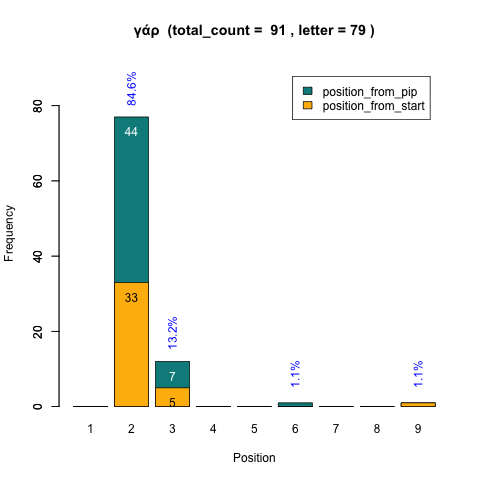
\includegraphics[width=1\linewidth]{paul_plots/par1_lt79.png}
\end{subfigure}
\caption{Frequency of particle ???(yap) at each absolute position in Pauline letters}
\end{figure}

\begin{figure}
\begin{subfigure}{0.45\textwidth}
\centering
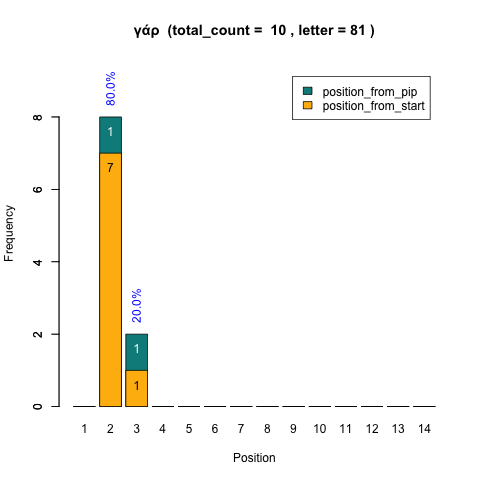
\includegraphics[width=1\linewidth]{peter_plots/par1_lt81.png}
\end{subfigure}
\begin{subfigure}{0.45\textwidth}
\centering
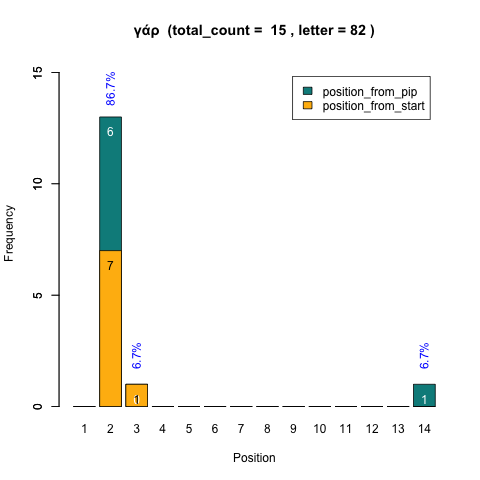
\includegraphics[width=1\linewidth]{peter_plots/par1_lt82.png}
\end{subfigure}
\caption{Frequency of particle ???(yap) at each absolute position in petrine letters}
\label{peter_yap}
\end{figure}

\section{References}
Black, Stephanie (2002), Sentence Conjunctions in the Gospel of Matthew: ???, ??, ????, ???, ???? and Asyndeton in Narrative Discourse. London \\

Denniston, J. D. (1954), The Greek Particles. Oxford. \\

Frischer, Bernard (1991): Shifting paradigms: new approaches to Horace�s Ars poetica. American classical studies. Scholars Press, 1991. isbn: 9781555406196. url: http: //books.google.de/books?id=T1F0AAAAIAAJ. \\ 

Thrall, Margaret Eleanor (1962) Greek Particles in the New Testament (Linguistic and Exegetical Studies 3). Leiden. \\

\end{document}
